\documentclass[draft, twocolumn]{article}
\usepackage[unicode,draft=false,hidelinks]{hyperref}
\usepackage{cite}
\usepackage{catchfilebetweentags}
\usepackage{amssymb}
\usepackage{turnstile}
\usepackage{bbm}
\usepackage[greek, english]{babel}
\usepackage{MnSymbol}
\usepackage{stmaryrd}
\usepackage{csquotes}
\newcommand\doubleplus{+\kern-1.3ex+\kern0.8ex}
\newcommand\mdoubleplus{\ensuremath{\mathbin{+\mkern-8mu+}}}
\makeatletter
\newcommand\incircbin
{%
  \mathpalette\@incircbin
}
\newcommand\@incircbin[2]
{%
  \mathbin%
  {%
    \ooalign{\hidewidth$#1#2$\hidewidth\crcr$#1\bigcirc$}%
  }%
}
\newcommand{\oeq}{\ensuremath{\incircbin{=}}}
\makeatother
\makeatletter
\newcommand\insquarebin
{%
  \mathpalette\@insquarebin
}
\newcommand\@insquarebin[2]
{%
  \mathbin%
  {%
    \ooalign{\hidewidth$#1#2$\hidewidth\crcr$#1\bigbox$}%
  }%
}
\newcommand{\sqtri}{\ensuremath{\insquarebin{\triangle}}}
\makeatother
\usepackage{ucs}
\DeclareUnicodeCharacter{8759}{\ensuremath{\squaredots}}
\DeclareUnicodeCharacter{951}{\textgreek{\texteta}}
\DeclareUnicodeCharacter{737}{\ensuremath{^\text{l}}}
\DeclareUnicodeCharacter{691}{\ensuremath{^\text{r}}}
\DeclareUnicodeCharacter{7523}{\ensuremath{_\text{r}}}
\DeclareUnicodeCharacter{8718}{\ensuremath{\blacksquare}}
\DeclareUnicodeCharacter{957}{\textgreek{\textnu}}
\DeclareUnicodeCharacter{961}{\textgreek{\textrho}}
\DeclareUnicodeCharacter{929}{\textgreek{\textRho}}
\DeclareUnicodeCharacter{954}{\textgreek{\textkappa}}
\DeclareUnicodeCharacter{10214}{\ensuremath{\lsem}}
\DeclareUnicodeCharacter{10215}{\ensuremath{\rsem}}
\DeclareUnicodeCharacter{8857}{\mdoubleplus}
\DeclareUnicodeCharacter{8860}{\oeq}
\DeclareUnicodeCharacter{9043}{\ensuremath{\sqtri}}
\DeclareUnicodeCharacter{928}{\textgreek{\textPi}}
\DeclareUnicodeCharacter{922}{\textgreek{\textKappa}}
\DeclareUnicodeCharacter{931}{\textgreek{\textSigma}}
\DeclareUnicodeCharacter{916}{\textgreek{\textDelta}}
\DeclareUnicodeCharacter{8779}{\ensuremath{\backtriplesim}}
\DeclareUnicodeCharacter{8799}{\ensuremath{\stackrel{?}{=}}}
\DeclareUnicodeCharacter{10181}{\ensuremath{\lbag}}
\DeclareUnicodeCharacter{10182}{\ensuremath{\rbag}}
\DeclareUnicodeCharacter{8760}{\ensuremath{-}}
\usepackage[utf8x]{inputenc}
\usepackage[T1]{fontenc}
\usepackage{autofe}
\usepackage[references]{agda}
\usepackage{bbding}
\setlength{\marginparwidth}{2cm}
\usepackage[obeyDraft]{todonotes}
\usepackage{lineno}
\setlength\linenumbersep{-0.5cm}
\usepackage{amsthm}
\theoremstyle{definition}
\newtheorem{definition}{Definition}[section]
\theoremstyle{definition}
\newtheorem{principle}{Principle}[section]
\usepackage{subcaption}
\usepackage{graphicx}
\usepackage{tikz}
\usetikzlibrary{decorations.pathmorphing}
\usetikzlibrary{snakes}
\usetikzlibrary{arrows}
\usetikzlibrary{cd}
\usepackage{forest}
\author{Donnacha Oisín Kidney}
\title{Automatically And Efficiently Illustrating Polynomial Equalities in Agda}
\begin{document}
\maketitle
\begin{abstract}
  We present a new library which automates the construction of equivalence
  proofs between polynomials over commutative rings and semirings in the
  programming language Agda\cite{norell_dependently_2008}. We use Agda's
  reflection machinery to provide a simple interface to the solver, and
  demonstrate a novel use of the constructed relations.
\end{abstract}
\tableofcontents
\section{Introduction}
Truly formal proofs of even basic mathematical identities are notoriously
tedious and verbose. Perhaps the canonical example is Russell and Whitehead's
proof that \(1+1=2\), which finally arrives on page 379 of Principia
Mathematica\cite{whitehead_principia_1910}. 

More modern systems have greatly simplified the underlying formalisms, but they
still often suffer from a degree of explicitness that makes even elementary
identities daunting. Dependently-typed programming languages like
Agda\cite{norell_dependently_2008} and
Coq\cite{the_coq_development_team_2018_1219885} are examples of such systems:
used in the naïve way, equivalence proofs require the programmer to specify
every individual step (``here we rely on the commutativity of \(+\), followed by
the associativity of \(\times\) on its right-hand-side'', and so on).

Coq and Agda are not just programming languages in name, though: they are
fully-fledged and powerful, capable of producing useful software, including
automated computer-algebra systems. Unlike most CASs, those written in Coq or
Agda come with added guarantees of correctness in their operation. Furthermore,
these systems can be used to automate the construction of identity proofs which
would otherwise be too tedious to do by hand.
\subsection{Related Work}
The state-of-the-art solver for polynomial equalities (over commutative rings)
was originally presented in\cite{gregoire_proving_2005}, and is used in Coq's
\verb+ring+ solver. This work improved on the already existing
solver\cite{Coq:manual} in both efficiency and flexibility. In both the old and
improved solvers, a reflexive technique is used to automate the construction of
the proof obligation (as described in\cite{boutin_using_1997}).

Agda\cite{norell_dependently_2008} is a dependently-typed programming language
based on Martin-Löf's Intuitionistic Type
Theory\cite{martin-lof_intuitionistic_1980}. Its standard
library\cite{danielsson_agda_2018} currently contains a ring solver which is
similar in flexibility to Coq's \verb+ring+, but doesn't support the
reflection-based interface, and is less efficient due to its use of a dense
(rather than sparse) internal data structure.

In\cite{geuvers_automatically_2017}, an implementation of an automated solver
for the dependently-typed language Idris\cite{brady_idris_2013} is described. It
uses type-safe reflection to provide a simple and elegant interface, and its
internal solver algorithm uses a correct-by-construction approach. The solver is
defined over \emph{non}commutative rings, however, meaning that it is more
general (can work with more types) but less powerful (meaning it can prove fewer
identities). It does not use a sparse representation.

Reflection and metaprogramming are relatively recent additions to Agda, but form
an important part of the interfaces to automated proof procedures. Reflection in
dependent types in general is explored in\cite{christiansen_practical_2015}, and
specific to Agda in\cite{van_der_walt_reflection_2012}.

The progress of various formalization efforts is charted
in\cite{wiedijk_formalizing_2018}. DoCon\cite{meshveliani_docon-provable_2018}
is a notable Agda library in this regard: its implementation and goal is
described in\cite{meshveliani_dependent_2013}. \cite{cheng_functional_2018}
describes the manipulation of polynomials in both Haskell and Agda.

Finally, the study of \emph{didactic} computer algebra systems is explored
in\cite{lioubartsev_constructing_2016}.
\subsection{Contributions}
\begin{description}
  \item[An New, Efficient Ring Solver]
    We provide an implementation of a polynomial solver which uses the same
    optimizations described in\cite{gregoire_proving_2005} in the programming
    language Agda.
  \item[Techniques For Efficient Verification] We demonstrate several techniques
    to thread verification and proof logic through algorithms \emph{without}
    changing complexity class. These techniques are of general use in functional
    languages with type systems powerful enough to express invariants.

    We also demonstrate a use of the Algebra of Programming approach in
    Agda\cite{mu_algebra_2009}.
  \item[A Simple Reflection-Based Interface] We use Agda's reflection machinery
    to provide the following interface to the solver:
    \ExecuteMetaData[Introduction.tex]{lemma}
    It imposes minimal overhead on the user: only the \(\AgdaDatatype{Ring}\)
    implementation is required, with no need for user implementations of
    quoting. Despite this, it is generic over any type which implements ring.
  \item[A Didactic Computer-Algebra System] As a result of the flexibility of
    the solver, the equivalence relation it constructs can be instantiated into
    a number of different forms (not just equality, for instance). While this
    has been exploited in Agda before to generate isomorphisms over containers,
    we use it here to construct didactic (or ``step-by-step'') solutions.
\end{description}
\section{Explaining The Reflexive Technique With Monoids}
Before jumping into commutative rings, we will first illustrate a general
technique for automatically constructing equivalence proofs over a simpler
algebra---\emph{monoids}.

\begin{definition}[Monoids]
  A monoid is a set equipped with a binary operation, \(\bullet\), and a
  distinguished element \(\epsilon\), such that the following equations hold:
  \begin{align}
    x \bullet (y \bullet z) &= (x \bullet y) \bullet z \tag{Associativity} \\
    x \bullet \epsilon      &= x \tag{Left Identity} \\
    \epsilon \bullet x      &= x \tag{Right Identity}
  \end{align}
  Addition and multiplication (with 0 and 1 being the respective identity
  elements) are perhaps the most obvious instances of the algebra. In computer
  science, monoids have proved a useful abstraction for formalizing concurrency
  (in a sense, an associative operator is one which can be evaluated in any
  order).
\end{definition}
\subsection{A ``Trivial'' Identity}
\begin{figure}[h]
  \ExecuteMetaData[Monoids.tex]{mon-ident}
  \caption{A Simple Identity Of Monoids}
  \label{mon-ident}
\end{figure}

As a running example for this section, we will use the identity in
figure~\ref{mon-ident}. To a human, the fact that the identity holds may well be
obvious: \(\AgdaField{∙}\) is associative, so we can scrub out all the
parentheses, and \(\AgdaField{ε}\) is the identity element, so scrub it out too.
After that, both sides are equal, so voilà! 

Unfortunately, our compiler isn't nearly that clever. As alluded to before, we
need to painstakingly specify every intermediate step, justifying every move:

\begin{samepage}
  \begin{linenumbers}
    \ExecuteMetaData[Monoids.tex]{mon-proof}
  \end{linenumbers}
\end{samepage}

The syntax is designed to mimic that of a handwritten proof: line 3 is the
expression on the left-hand side of \(\AgdaField{≈}\) in the type, and line 9
the right-hand-side. In between, the expression is repeatedly rewritten into
equivalent forms, with justification provided inside the angle brackets. For
instance, to translate the expression from the form on line 3 to that on line 5,
the associative property of \(\AgdaField{∙}\) is used on line 4.

One trick worth pointing out is on line 6: the \(\AgdaFunction{∙-cong}\) lifts
two equalities to either side of a \(\AgdaField{∙}\). In other words, given a
proof that \(x_1 \; \AgdaField{≈} \; x_2\), and \(y_1 \; \AgdaField{≈} \; y_2\),
it will provide a proof that \(x_1 \; \AgdaField{∙} \; y_1 \; \AgdaField{≈} \;
x_2 \; \AgdaField{∙} \; y_2\). This function needs to be explicitly provided by
the user, as we only require \(\AgdaField{≈}\) to be an equivalence relation
(not just propositional equality). In other words, we don't require it to be
substitutive.
\subsection{ASTs for the Language of Monoids}
The first hurdle for automatically constructing proofs comes from the fact that
the identity is opaque: it's hidden behind a lambda. We can't scrutinize or
pattern-match on its contents. Our first step, then, is to define an AST for
these expressions which we \emph{can} pattern-match on:

\begin{samepage}
  \ExecuteMetaData[Monoids.tex]{mon-ast}
\end{samepage}

We have constructors for both monoid operations, and a way to refer to
variables. These are referred to by their de Bruijn indices (the type itself is
indexed by the number of variables it contains). Here is how we would represent
the left-hand-side of the identity in figure~\ref{mon-ident}:
\ExecuteMetaData[Monoids.tex]{lhs-ast}

To get \emph{back} to the original expression, we can write an ``evaluator'':
\ExecuteMetaData[Monoids.tex]{eval-ast}

This performs no normalization, and as such its refult is \emph{definitionally}
equal to the original expression\footnotemark:
\footnotetext{
  The type of the unnormalized expression has changed slightly: instead of being
  a curried function of \(n\) arguments, it's now a function which takes a
  vector of length \(n\). The final solver has an extra translation step for
  going between these two representations, but it's a little fiddly, and not
  directly relevant to what we're doing here, so we've glossed over it. We refer
  the interested reader to the Relation.Binary.Reflection module of Agda's
  standard library\cite{danielsson_agda_2018} for an implementation.
}
\ExecuteMetaData[Monoids.tex]{eval-nonnorm}

We've thoroughly set the table now, but we still don't have a solver. What's
missing is another evaluation function: one that normalizes.
\subsection{Canonical Forms}
In both the monoid and ring solver, we will make use of the \emph{canonical
  forms} of expressions in each algebra. Like the AST we defined above, these
canonical forms represent expressions in the algebra, however \emph{unlike} the
AST, they definitionally obey the laws of the algebra. 

For monoids, the canonical form is \emph{lists}.

\ExecuteMetaData[Monoids.tex]{list-def}

\(\AgdaField{ε}\) here is simply the empty list, and \(\AgdaField{∙}\) is
concatenation:
\ExecuteMetaData[Monoids.tex]{list-monoid}

Similarly to the previous AST, it has variables and is indexed by the number of
variables it contains. Its evaluation will be recognizable to functional
programmers as the \(\AgdaFunction{foldr}\) function:
\ExecuteMetaData[Monoids.tex]{list-eval}

And finally (as promised) the opening identity is \emph{definitionally} true
when written in this language:
\ExecuteMetaData[Monoids.tex]{list-obvious}

Now, to ``evaluate'' a monoid expression in a \emph{normalized} way, we simply
first convert to the language of lists:
\ExecuteMetaData[Monoids.tex]{ast-norm}

Or, combining both steps into one:
\ExecuteMetaData[Monoids.tex]{ast-norm-interp}
\subsection{Homomorphism}
\begin{figure*}
  \makebox[\textwidth][c]{
    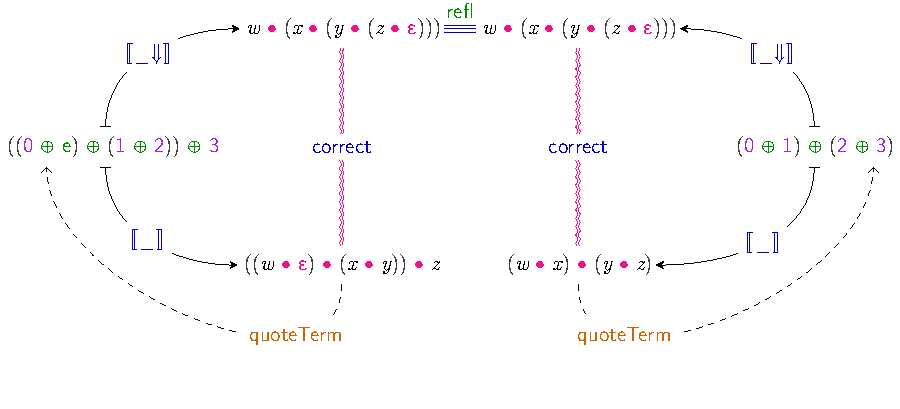
\includegraphics[draft=false]{graphics/reflexive-process}
  }
  \caption{The Reflexive Proof Process}
  \label{proof-process}
\end{figure*}
Now we have a concrete way to link the normalized and non-normalized forms of
the expressions. A diagram of the strategy for constructing our proof is in
figure~\ref{proof-process}. The goal is to construct a proof of equivalence
between the two expressions at the bottom: to do this, we first construct the
AST which represents the two expressions (for now, we'll assume the user
constructs this AST themselves. Later we'll see how too construct it
automatically from the provided expressions). Then, we can evaluate it into
either the normalized form, or the unnormalized form. Since the normalized forms
are syntactically equal, all we need is \(\AgdaInductiveConstructor{refl}\) to
prove their equality. The only missing part now is \(\AgdaFunction{correct}\),
which is the task of this section.

Taking the non-normalizing interpreter as a template, the three cases are as
follows\footnotemark:
\begin{align}
  \AgdaFunction{⟦} \; x \; \AgdaInductiveConstructor{⊕} \; y \; \AgdaFunction{⟧} \; \rho \; &\AgdaField{≈} \; \AgdaFunction{⟦} \; x \; \AgdaInductiveConstructor{⊕} \; y \; \AgdaFunction{⇓⟧} \; \rho \label{plus-hom} \\
  \AgdaFunction{⟦}      \; \AgdaInductiveConstructor{e}      \; \AgdaFunction{⟧} \; \rho \; &\AgdaField{≈} \; \AgdaFunction{⟦}      \; \AgdaInductiveConstructor{e}      \; \AgdaFunction{⇓⟧} \; \rho \label{e-hom}    \\
  \AgdaFunction{⟦}      \; \AgdaInductiveConstructor{ν} \; i \; \AgdaFunction{⟧} \; \rho \; &\AgdaField{≈} \; \AgdaFunction{⟦}      \; \AgdaInductiveConstructor{ν} \; i \; \AgdaFunction{⇓⟧} \; \rho \label{var-hom}
\end{align}
\footnotetext{
  Equations \ref{plus-hom} and \ref{e-hom} comprise a monoid
  homomorphism.
}

Proving each of these cases in turn finally verifies the correctness of our list
language.
\ExecuteMetaData[Monoids.tex]{correct-ast}
\subsection{Usage}
Combining all of the components above, with some plumbing provided by the
\(\AgdaModule{Relation.Binary.Reflection}\) module, we can finally automate the
solving of the original identity in figure~\ref{mon-ident}:
\ExecuteMetaData[Monoids.tex]{ident-auto-proof}
\subsubsection{Reflection}
While the procedure is now automated, the interface isn't ideal: users have to
write the identity they want to prove \emph{and} the AST representing the
identity. Removing this step is the job of reflection
(section~\ref{reflection}): in figure~\ref{proof-process} it's represented by
the path labeled \(\AgdaKeyword{quoteTerm}\).
\section{A Polynomial Solver}
We now know the components required for an automatic solver for some algebra: a
canonical form, a concrete representation of expressions, and a proof of
correctness (homomorphism). We now turn our focus to polynomials.
\subsection{Choice of Algebra}
So far, we've assumed the solver is defined over commutative rings. That wasn't
the only algebra available to us when writing a solver, though: we've
demonstrated techniques using monoids in the previous section, and
indeed\cite{geuvers_automatically_2017} uses \emph{non}commutative rings as its
algebra. Here, we will justify our\footnotemark choice (and admit to a minor lie).
\footnotetext{
  ``Our'' choice here is the same choice as in\cite{gregoire_proving_2005}.
}

Because we want to solve arithmetic equations, we will need the basic operations
of addition, multiplication, subtraction, and exponentiation (to a power in
\(\mathbb{N}\)). This is only half of the story, though: along with those
operations we will need to specify the laws or equations that they obey
(commutativity, associativity, etc.). Here we need balance: the more equations
specified, the more equalities the solver can prove, but the fewer types the
solver will be available for.

The elephant in the room here is \(\mathbb{N}\): perhaps the most used numeric
type in Agda, it doesn't have an additive inverse. So that our solver will still
function with it as a carrier type, we don't require
\[x - x = 0\]
to hold. This lets us lawfully define negation as the identity function for
\(\mathbb{N}\).

A potential worry is that because we don't require \(x - x = 0\)
axiomatically, it won't be provable in our system. This is not so: as is pointed
out in\cite{gregoire_proving_2005},as long as \(1 - 1\) reduces to \(0\) in the
coefficient set, the solver will verify the identity.
\subsection{Horner Normal Form}
The canonical representation of polynomials is a list of coefficients, least
significant first (``Horner Normal Form''). Our initial attempt at encoding this
representation will begin like so:
\ExecuteMetaData[HornerNormalForm.tex]{opening}
The entire module is parameterized by the choice of coefficient. This
coefficient should support the ring operations, but it is ``raw'', i.e. it
doesn't prove the ring laws. The operations\footnotemark on the polynomial
itself are defined in figure~\ref{simple-ops}.
\footnotetext{
  Symbols chosen for operators use the following mnemonic:
  \begin{enumerate}
    \item Operators preceded with ``\(\mathbb{N}.\)'' are defined over
      \(\mathbb{N}\); e.g. \(\mathbb{N}.+\), \(\mathbb{N}.*\).
    \item Plain operators, like \(+\) and \(*\), are defined over the
      coefficients.
    \item Boxed operators, like \(\boxplus\) and \(\boxtimes\), are defined over
      polynomials.
  \end{enumerate}
}

\begin{figure}
  \ExecuteMetaData[HornerNormalForm.tex]{impl}
  \caption{
    Simple Operations on Dense Horner Normal Form}
  \label{simple-ops}
\end{figure}
Finally, evaluation of the polynomial uses ``Horner's rule'' to minimize
multiplications:
\ExecuteMetaData[HornerNormalForm.tex]{eval}
\subsection{Eliminating Redundancy}
As it stands, the above representation has two problems:

\begin{description}
  \item[Redundancy] The representation suffers from the problem of trailing
    zeroes. In other words, the polynomial $2x$ could be represented by any of
    the following:
  
    \begin{align*}
      & 0, 2 \\
      & 0, 2, 0 \\
      & 0, 2, 0, 0 \\
      & 0, 2, 0, 0, 0, 0, 0
    \end{align*}
    
    This is a problem for a solver: the whole \emph{point} is that equivalent
    expressions are represented the same way.

  \item[Inefficiency] Expressions will tend to have large gaps, full only of
    zeroes. Something like $x^5$ will be represented as a list with 6 elements,
    only the last one being of interest. Since addition is linear in the length
    of the list, and multiplication quadratic, this is a major concern.
\end{description}

In\cite{gregoire_proving_2005}, the problem is addressed primarily from the
efficiency perspective: they add a field for the ``power index''. For our case,
we'll just store a list of pairs, where the second element of the pair is the
power index\footnote{
  In\cite{gregoire_proving_2005}, the expression \((c , i) \squaredots P\)
  represents \(P \times X^i + c\). We found that \(X^i \times (c + X \times P)\)
  is a more natural translation, and it's what we use here. A power index of
  \(i\) in this representation is equivalent to a power index of \(i+1\)
  in\cite{gregoire_proving_2005}.
}.

As an example, the polynomial:
\[ 3 + 2x^2 + 4x^5 + 2x^7 \]
Will be represented as:
\[ (3,0),(2,1),(4,2),(2,1) \]
Or, mathematically:
\[ x^0 (3 + x x^1 (2 + x x^2 * (4 + x x^1 (2 + x 0)))) \]

\begin{definition}[Dense and Sparse Encodings]
  In situations like this, where inductive types have large ``gaps'' of
  zero-like terms between interesting (non-zero-like) terms, the encoding which
  uses an index to represent the distance to the next interesting term will be
  called \emph{sparse}, and the encoding which simply stores the zero term will
  be called \emph{dense}.
\end{definition}
\subsubsection{Uniqueness}
While this form solves our efficiency problem, we still have redundant
representations of the same polynomials. In\cite{gregoire_proving_2005}, care
is taken to ensure all operations include a normalizing step, but this is not
verified: in other words, it is not proven that the polynomials are always in
normal form.

Expressing that a polynomial is in normal form turns out to be as simple as
disallowing zeroes: without them, there can be no trailing zeroes, and all gaps
must be represented by power indices. To check for zero, we require the user
supply a decidable predicate on the coefficients. This changes the module
declaration like so:
\ExecuteMetaData[EliminatingRedundancy.tex]{opening}

Importantly, we don't require that the user provides a decidable proof of
\emph{equivalence}, rather just a decidable proof of some predicate which can
later be translated into an equivalence with zero. Functionally, this means the
user could supply a predicate which is always false, or a predicate which is
only \emph{weakly} decidable.

And now we have a definition for sparse polynomials:
\ExecuteMetaData[EliminatingRedundancy.tex]{decl}

The proof of nonzero is marked irrelevant (preceded with a dot) to avoid
computing it at runtime.

We can wrap up the implementation with a cleaner interface by providing a
normalizing version of \(\AgdaInductiveConstructor{\_∷\_}\):
\ExecuteMetaData[EliminatingRedundancy.tex]{norm-cons}
\subsection{A Sparse Encoding for Multiple Variables}
So far, the polynomials have been (suspiciously) single-variable. Luckily,
there's a natural technique to support multiple variables: for a polynomial with
$n$ variables, it has coefficients of $n-1$ variables. In types:
\ExecuteMetaData[SparseMulti.tex]{dense-poly}

However, this encoding is again a dense one. In a polynomial of $n$ variables,
addressing the $n^{th}$ variable needlessly requires $n-1$ layers of nesting.
Alternatively, a constant expression in this polynomial is hidden behind $n$
layers of nesting.

In contrast to the previous sparse encoding, though, the size of the gap is
type-relevant. Because the polynomial types are \emph{indexed} by the number of
variables they contain, storing a simple \(\AgdaDatatype{ℕ}\) won't carry enough
information to properly type the resulting operations. Instead, we need to store
the size of the inner and outer polynomial, and a proof that the inner
polynomial does indeed have fewer variables than the outer.
\ExecuteMetaData[SparseMulti.tex]{sparse-poly}

We will defer the description of the implementation of \(\leq\) for now.
\subsection{Efficiency in Indexed Types}
\subsubsection{Call-Pattern Specialization}
While both sparse encodings provide a more space-efficient representation, the
computational efficiency has yet to be realized. Starting with the sparse
monomial, we'll look at the addition function to start off. In the dense
encoding (figure~\ref{simple-ops}), we needed to line up corresponding
coefficients to add together. For this encoding, the ``corresponding''
coefficients are slightly harder to find. In order to line things p correctly,
we'll need to compare the gap indices. This, however, presents our first
problem:
\ExecuteMetaData[EliminatingRedundancy.tex]{nonterm-add}
The above definition won't pass the termination checker. While it does indeed
terminate, it isn't structurally decreasing in its arguments. To argue our case
that the function does terminate, we have to reveal this fact to the compiler
using a well-known optimization for functional languages called ``call-pattern
specialization''\cite{jones_call-pattern_2007}.
\begin{principle}[To make termination obvious, perform call-pattern
    specialization]
  Unpack any constructors into function arguments as soon as possible, and
  eliminate any redundant pattern matches in the offending functions. Happily,
  this transformation both makes termination more obvious \emph{and} improves
  performance.

  This transformation is performed automatically by GHC as an optimization:
  perhaps a similar transformation could be performed by Agda's termination
  checker to reveal more terminating programs.
\end{principle}

For our case, the principle applied can be seen in figure~\ref{term-add}.

\begin{figure*}
  \centering
  \ExecuteMetaData[EliminatingRedundancy.tex]{term-add}
  \caption{Termination by Call-Pattern Specialization}
  \label{term-add}
\end{figure*}

\subsubsection{Built-In Functions}
The second optimization we might rely on involves the call to
\(\AgdaFunction{compare}\). This is a classic ``leftist'' function: it returns
an \emph{indexed} data type:

\ExecuteMetaData[EfficiencyInIndexedTypes.tex]{ord-type}

The compare function itself is \(\mathcal{O}(\min(n, m))\):

\ExecuteMetaData[EfficiencyInIndexedTypes.tex]{cmp-impl}

The implementation of \(\AgdaFunction{compare}\) may raise suspicion with
regards to efficiency: if this encoding of polynomials improves time complexity
by skipping the gaps, don't we lose all of that when we encode the gaps as Peano
numbers?

The answer is a tentative no. Firstly, since we are comparing gaps, the
complexity can be no larger than that of the dense implementation. Secondly, the
operations we're most concerned about are those on the underlying coefficient;
and, indeed, this sparse encoding does reduce the number of those significantly.
Thirdly, if a fast implementation of \(\AgdaFunction{compare}\) is really and
truly demanded, there are tricks we can employ.

Agda has a number of built-in functions on the natural numbers: when applied to
closed terms, these call to an implementation on Haskell's \texttt{Integer}
type, rather than the unary implementation. For our uses, the functions of
interest are \(\AgdaFunction{-}\), \(\AgdaFunction{+}\), \(\AgdaFunction{<}\),
and \(\AgdaFunction{==}\). The comparison functions provide booleans rather than
evidence, but we can prove they correspond to the evidence-providing versions:
\ExecuteMetaData[EfficiencyInIndexedTypes.tex]{fast-cmp-hom}
Combined with judicious use of \(\AgdaFunction{erase}\) and
\(\AgdaFunction{inspect}\), we get the implementation which can be seen in
figure~\ref{fast-cmp}.

\begin{figure*}
  \centering
  \ExecuteMetaData[EfficiencyInIndexedTypes.tex]{fast-cmp}
  \caption{Fast comparison function using built-in functions on the natural
    numbers}
  \label{fast-cmp}
\end{figure*}
\subsubsection{Hanging Indices}
Finally we return to the unprovided definition of \(\leq\) above. As we saw with
the exponent indices, we will eventually need to compare gaps. Unlike before,
though, the evidence provided by the comparison function will have to mesh
properly with this \(\leq\) proof. In other words, after comparing the two
indices, we'll need to get another proof bundled with the evidence that one is
less than another.

\subsection{Abstraction and Folds for Simpler Proofs}
\subsection{Proving Higher-Order Termination With Well-Founded Recursion}
\section{Reflection} \label{reflection}
\section{Setoid Applications}
\subsection{Isomorphisms}
\subsection{Didactic Solutions}
\section{The Correct-By-Construction Approach}
\bibliographystyle{IEEEtranS}
\bibliography{bibliography.bib}
\end{document}